\documentclass{article}

% set font encoding for PDFLaTeX or XeLaTeX
\usepackage{ifxetex}
\ifxetex
  \usepackage{fontspec}
\else
  \usepackage[T1]{fontenc}
  \usepackage[utf8]{inputenc}
  \usepackage{lmodern}
  \usepackage{graphicx}
  \usepackage{wrapfig}
\fi



% used in maketitle
\title{La atmósfera terrestre}
\author{Mariana Ruíz Quintín}



% Enable SageTeX to run SageMath code right inside this LaTeX file.
% documentation: http://mirrors.ctan.org/macros/latex/contrib/sagetex/sagetexpackage.pdf
% \usepackage{sagetex}

\begin{document}
\maketitle

\begin{figure}
   \caption{Atmósfera de la Tierra}
   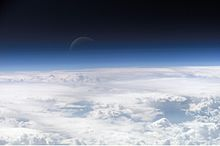
\includegraphics[width=0.5\textwidth]{Top_of_Atmosphere.jpg}%Notaalpiedeimagen
   \centering
   \label{Atmósfera de la Tierra}%Etiqueta
  \end{figure}
  
 
  
\section{Introducción}

 
La atmósfera terrestre está constituida por distintos gases, los cuales comunmente son conocidos como aire, y rodean completamente el planeta siendo retenidos por la gravedad de éste mismo. Por consecuencia, la vida en la Tierra permanece protegida de la radiación proveniente del sol y el agua aparece en sus tres estados, lo cual se debe a la presión generada por la atmósfera. 
  Los gases que conforman la atmósfera son el nitrógeno, oxígeno, argón, dióxido de carbono, entre otros gases. El porcentaje que corresponde a la cantidad de éstos gases es de 78.09\%, 20.95\%, 0.93\% y 0.04\% respectivamente.
Tres cuartas partes de la atmósfera están dentro de unos 11 km de la superficie. Se vuelve más delgada a medida que aumenta la altitud, sin un límite definido entre la atmósfera y el espacio exterior. La línea de Kármán, a 100 km (62 mi), o 1.57\% del radio de la Tierra, se usa a menudo como el límite entre la atmósfera y el espacio exterior. Los efectos atmosféricos se hacen evidentes durante la reentrada atmosférica de naves espaciales a una altitud de alrededor de 120 km. Varias capas se pueden distinguir en la atmósfera, en función de características tales como la temperatura y la composición. El estudio de la atmósfera de la Tierra y sus procesos se llama ciencia atmosférica (aerología).
  
  
  
  
\section{Composición}

Los principales elementos constituyentes de la atmósfera son el nitrógeno, el oxígeno y el argón. Los gases restantes que se encuentran son los gases de efecto invernadero, principalmente dióxido de carbono, metano, óxido nitroso y ozono. Varios contaminantes industriales también pueden estar presentes en forma de gases o aerosoles, como cloro, compuestos de flúor y vapor de mercurio elemental. 

\section{Estructura de la atmósfera}

\subsection{Capas principales}

En general, la presión el aire y densidad decrece con altitud en la atmósfera. Sin embargo, la temperatura tiene un perfil más complicado con la altitud, y puede permanecer relativamente constante o incluso aumentar con la altitud en algunas regiones.  La atmósfera de la Tierra se puede dividir en cinco capas principales. Las cuales son:


\subsubsection{EXOSFERA de 700 a 10,000 km (440 a 6,200 millas)}
  Esta capa está compuesta en principio por densidades bastante bajas de hidrógeno, helio y varias moléculas más pesadas. Los átomos y moléculas están tan separados que pueden viajar cientos de kilómetros sin colisionar entre sí. 
\subsubsection{TERMOSFERA de 80 a 700 km (50 a 440 millas)}
  La temperatura de esta capa aumenta gradualmente con la altura. A diferencia de la estratosfera debajo de ella, en donde una inversión de temperatura se debe a la absorción de radiación por el ozono, la inversión en la termosfera ocurre debido a la extremadamente baja densidad de sus moléculas. 
\subsubsection{MESOSFERA 50 a 80 km (31 a 50 millas)}
La mesosfera es la tercera capa más alta de la atmósfera del planeta, ocupando la región sobre la estratosfera y debajo de la termosfera. Las temperaturas caen con el aumento de la altitud a la mesopausia que marca la parte superior de esta capa media de la atmósfera. Es el lugar más frío de la Tierra y tiene una temperatura promedio de -85 grados Celsius. 
\subsubsection{ESTRATOSFERA 12 a 50 km (7 a 31 millas)}
La presión atmosférica en la parte superior de la estratosfera es aproximadamente 1/1000 de la presión al nivel del mar. Contiene la capa de ozono, que es la parte de la atmósfera de la Tierra que contiene concentraciones relativamente altas de ese gas. La estratosfera define una capa en la que las temperaturas aumentan con el aumento de la altitud. 
\subsubsection{TROPOSFERA de 0 a 12 km (de 0 a 7 millas)}
 La troposfera es la capa más baja de la atmósfera de la Tierra y se extiende desde la superficie de la Tierra hasta una altura promedio de aproximadamente 12 km. Dicha capa está delimitada arriba por la tropopausa, un límite marcado en la mayoría de los lugares por una inversión de temperatura.
 
 
\subsection{Otras capas}

Dentro de las cinco capas principales que están determinadas en gran medida por la temperatura, varias capas secundarias se pueden distinguir por otras propiedades:

La capa de ozono está contenida dentro de la estratosfera. Alrededor del 90\% del ozono en la atmósfera de la Tierra está contenido en la estratosfera. La ionosfera es una región de la atmósfera ionizada por la radiación solar. Es responsable de auroras. Durante el día, se extiende de 50 a 1,000 km e incluye la mesosfera, la termosfera y partes de la exosfera. La homósfera y la heterosfera se definen según si los gases atmosféricos están bien mezclados. La homosfera basada en la superficie incluye la troposfera, la estratosfera, la mesosfera y la parte más baja de la termosfera. Sobre esta altitud se encuentra la heterosfera, que incluye la exosfera y la mayor parte de la termosfera. Aquí, la composición química varía con la altitud. La parte superior de la heterosfera está compuesta casi por completo de hidrógeno.





\section{Propiedades físicas}

\subsection{Presión y espesor}
La presión atmosférica promedio a nivel del mar está definida por la Atmósfera Estándar Internacional como 101,325 pascales. Esto a veces se conoce como una unidad de atmósferas estándar (atm).

\subsection{Temperatura y velocidad del sonido}

 La temperatura disminuye con la altitud comenzando al nivel del mar, pero las variaciones en esta tendencia comienzan por encima de los 11 km, donde la temperatura se estabiliza a través de una gran distancia vertical a través del resto de la troposfera.
 Debido a que en un gas ideal de composición constante, la velocidad del sonido depende únicamente de la temperatura y no de la presión o densidad del gas, la velocidad del sonido en la atmósfera con la altitud adquiere la forma del perfil de temperatura complicado, y no refleja los cambios altitudinales en la densidad o la presión.
 
 \begin{figure}
   \caption{Temperatura de la Atmósfera}
   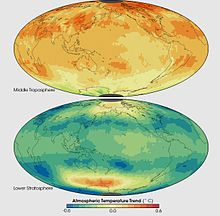
\includegraphics[width=0.5\textwidth]{Atmospheric_Temperature_Trend.jpg}%Notaalpiedeimagen
   \centering
   \label{Atmósfera de la Tierra}%Etiqueta
  \end{figure}

\subsection{Densidad y masa}

La densidad del aire a nivel del mar es de 1.2 kg / m3. La densidad no se mide directamente, pero se calcula a partir de mediciones de temperatura, presión y humedad utilizando la ecuación de estado para el aire. La masa promedio de la atmósfera es de aproximadamente 5 cuatrillones de toneladas.

\section{Propiedades ópticas}

La radiación solar es la energía que recibe la Tierra del sol y la Tierra también emite radiación hacia el espacio, pero a longitudes de onda más largas que no podemos ver. Parte de la radiación entrante y emitida es absorbida o reflejada por la atmósfera. 

\subsection{Dispersión}

Cuando la luz pasa a través de la atmósfera de la Tierra, los fotones interactúan con ella a través de la dispersión. Si la luz no interactúa con la atmósfera, se llama radiación directa y es lo que se vería si mirara directamente al Sol. La radiación indirecta es luz que se ha dispersado en la atmósfera.

\subsection{Absorción}

Diferentes moléculas absorben diferentes longitudes de onda de radiación. Cuando una molécula absorbe un fotón, aumenta la energía de la molécula. Esto calienta la atmósfera, pero la atmósfera también se enfría al emitir radiación. 

\subsection{Emisión}

La emisión es lo opuesto a la absorción, es cuando un objeto emite radiación. Los objetos tienden a emitir cantidades y longitudes de onda de radiación dependiendo de sus curvas de emisión de "cuerpo negro", por lo tanto, los objetos más calientes tienden a emitir más radiación, con longitudes de onda más cortas. 


\subsection{Índice de refracción}

El índice de refracción del aire es cercano, pero apenas superior a 1. Las variaciones sistemáticas en el índice de refracción pueden conducir a la flexión de los rayos de luz en recorridos ópticos largos. Este índice depende de la temperatura, causando refracción cuando el gradiente de temperatura es grande.

\section{Circulación}

La circulación atmosférica es el movimiento de aire a gran escala a través de la troposfera, y los medios por los cuales se distribuye el calor alrededor de la Tierra. La estructura a gran escala de la circulación atmosférica varía de un año a otro.


\begin{figure}
   \caption{Corrientes de aire}
   \includegraphics[width=0.45\textwidth]{220px-AtmosphCirc2.png}%Notaalpiedeimagen
   \centering
   \label{Atmósfera de la Tierra}%Etiqueta
  \end{figure}
  
  \section{Bibliografía}
  
  Atmosphere of Earth.(2018, 28 de Enero). Obtenido de https://en.wikipedia.org/wiki/Atmosphere\_of\_Earth
  


%¿Qué fue lo que más te llamó la atención de esta actividad? 
% Que trabajamos con un artículo en otro idioma, ya que no lo había hecho en alguna otra materia.
%¿Qué fue lo que se te hizo menos interesante?
% Nada, el tema es interesante.
%¿Qué cambios harías para mejorar esta actividad? 
% Nada.
%¿Cuál es tu primera impresión de uso de LATEX?
% Me parece algo complejo, porque no estoy familiarizada y además no se bien como hacer algunas cosas.
%¿El tiempo sugerido para esta actividad fue suficiente? 
%  Sí.
%¿Encontraste algún documento o recurso en línea útil que quisieras compartir con los demás?
% No.


\end{document}
